\documentclass[a4paper,14pt]{extreport}

%CONVENIENT COMMANDS
\newcommand{\bv}[1]{\hat{b_{#1}}}
\newcommand{\nv}[1]{\hat{n_{#1}}}
\newcommand{\vk}[1]{\prescript{#1}{}{\hat{v_k}}}

%PACKAGES
%Graphics
\usepackage{graphicx}
\graphicspath{ {./images/} }
%Math
\usepackage{mathtools}
\usepackage{amsmath}
\usepackage{bm}

%DOCUMENT START
\title{Attitude with an Attitude \\
\large An Informal Intro to Spacecraft Attitude Determination}
\author{Brian Leung\\University of Michigan, Class of 2022}

\begin{document}
\maketitle
\setcounter{tocdepth}{0}
\tableofcontents{}
\chapter{Preface}
\section{Prerequisites}
You're welcome to dive in and learn as you go, but knowing some \textbf{Physics 1/Dynamics}, \textbf{Calculus 1-3, Diff Eq} and \textbf{Linear Algebra} will help immensely. Honestly, with how applicable it is, you should just learn linear algebra in general. Classes at the undergraduate level should more than enough. If you're dedicated enough, there's also plenty of online classes that you can take.

\section{Message to the Reader}
At the time of writing this, I am not a seasoned spacecraft engineer nor a cutting edge researcher (well, fingers crossed). For now, I'm just a green undergrad in Aerospace Engineering, hoping that my understanding  will help you out. I hope you learn something new and feel a little more comfortable in this field.

\section{Acknowledgement}
I owe much thanks to CU Boulder's ``Spacecraft Dynamics and Control Specialization" on Coursera, and Professor Hanspeter Schaub, the professor of the course. Seriously, it's great. If you've got the time and access, I highly recommend you look through it.

\section{What This Text Offers}
I want to emphasize that this text is \underline{not} a university textbook level reference, bursting at the seams with advanced terminology and derivations. This will not delve into dynamic attitude determination or control theory either. 

This text is essentially CU Boulder's Specialization, Part 1, distilled down to the key takeaways. This gives a quick and dirty intro to the fundamentals of spacecraft attitude description and determination, minimizing lengthy proofs and derivation.\footnote{TLDR: attitude determination speedrun any \% glhf} It offers conceptual questions along the way to test your knowledge. It can act as a springboard into more advanced topics for the aspiring spacecraft engineer.

\chapter{What is Attitude Anyways?}

\section{Definition}
Hint: It's not a state of mind. A fairly straightforward definition for attitude is:

\begin{center}
\textbf{ATTITUDE: A body's angular orientation with respect to a reference frame.}
\end{center}

A body just refers to something like a plane, spacecraft, or satellite. Angular orientation? Pretty self-explanatory. The important part of this definition is the reference frame. 

Let me pose this question to you. If you're floating around in an infinite black void, how do you decide which way is up? or down? Of course, the problem is a bit more complex than that, but it's a question you can't answer without the help of a \textit{reference frame}.

\section{Frames?}

When I say reference frame, or frames in general, I mean coordinate frames: XYZ, \(\hat{i}\hat{j}\hat{k}\), 3 basis vectors, etc. You can pretty much glue a coordinate frame onto anything your heart desires. Attaching frames to things helps ground them in a mathematical context, and that helps in more reasons than I can name. For example, it's a lot easier to say things like "I'm about 10 meters south and 1 meter east of you with respect to your NED frame". This is just a rough example, but there are plenty of other good reasons to put frames on bodies.

\begin{center}
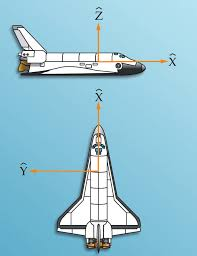
\includegraphics[width=4cm]{shuttle_body_frame}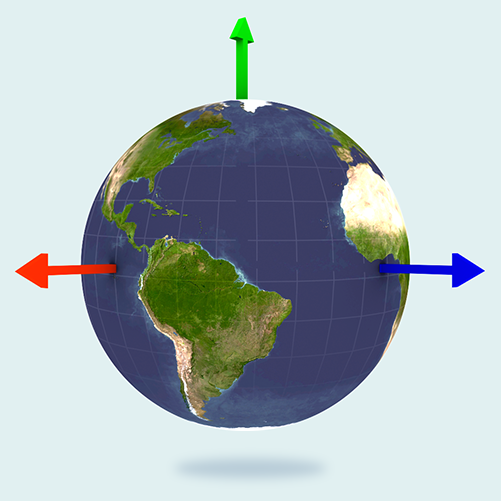
\includegraphics[height=5.2cm]{ecef}\\
A Frame on the Space Shuttle (L) \\ ECEF (Earth Centered, Earth Fixed) Frame (R)
\end{center}
\textbf{BODY: Refers to object of interest (e.g. spacecraft, satellite)}\\
When someone says "Body Frame", that refers to the frame glued to your satellite, space shuttle, UFO, rover. Basically, the thing you're trying to keep track of.\\\\
\textbf{INERTIAL: Refers to reference (e.g. Earth)}\\
When someone says inertial frame, they always mean reference. In most basic problems, the Earth and its variety of frames is what you'll refer to as inertial. However, you can also set the inertial frame to something that's not the Earth, like the ISS.\\

\section{It's All Relative}
I must emphasize that \emph{attitude is all relative}. Without knowing and specifying a reference frame, the description of your attitude is basically useless. 

\section{Why Worry About Attitude Anyways?}
Asking why attitude as important is similar to asking "Why do planes have to be headed in the right direction?". Depending on the project/mission, the importance of making sure the body is pointed in a desired direction ranges anywhere from marginal (super basic cubesats) or critical (space telescopes, comms satellites, space shuttle). But 9 times out of 10, attitude is pretty high on the priority list. This topic also has plenty of appearances outside of the aero sphere, such as in video games, robotics, computer vision, and biomechanics.

\section{4 Basic Truths}
\begin{enumerate}
\item \textbf{You need a minimum of 3 coordinates to describe relative angular displacement in 3D.} 

There's likely some in-depth proof showing why this is the case, but I'm not qualified enough to comment on it. The most popular example of a 3 coordinate set is Euler Angles.

\item \textbf{A 3 coordinate set will have at least 1 geometric orientation where the coordinates are \underline{singular}.} 

When an attitude description becomes \textbf{singular}, it's best described as acting ... weird. As in, the math doesn't behave very nicely (divisions by 0, non-uniqueness, etc.). As a real life example, think gimbal lock. The gimbal, when turned a certain way, loses degrees of freedom.

\item \textbf{At/near the singularities, the kinematic differential equations are also singular.} 

When you get close to a singularity in your attitude description, the kinematic differential equations of your attitude description also turn feral. These won't be too heavily covered in this text so don't worry too much about them.

\item \textbf{There exists redundant sets of 4 or more coordinates that are universally valid.}

\end{enumerate}
\chapter{DCM}

It doesn't stand for dichloromethane. And please, don't call it a DCM matrix.

\begin{center}
\textbf{DIRECTION COSINE MATRIX: A transformation matrix that converts from one reference frame to another.}
\end{center}

We consider the DCM the ``mother of all attitude parameterizations", quoting Professor Schaub. When I mean \emph{attitude parameterization}, I mean descriptions of your attitude, such as quaternions, Euler angles, etc. Every DCM maps to a parameterization of your choice and every parameterization maps back to a DCM. You could say it's the center of the great web of parameterizations. With DCMs, we directly interact with the basis vectors of the frames themselves. Before we move any further, let's get some \emph{formalisms} out of the way.
\section{Funky Formalisms}
When describing the body frame, I'll use the letter $b$. Describing the basis vectors that make up the body frame, I'll say $\bv{1}, \bv{2}, \bv{3}$. Likewise, describing the inertial frame basis vectors uses the letter $n$, like so: $\nv{1}, \nv{2}, \nv{3}$. Constantly writing out $\bv{1}, \bv{2}, \bv{3}$ is gonna get old real fast, so lets save our hands some work and assemble them into something called a \emph{vectrix}.
\[
\{\hat{b}\} = 
\begin{bmatrix}
\bv{1}\\ \bv{2}\\ \bv{3}\\
\end{bmatrix}\;
\{\hat{n}\} = 
\begin{bmatrix}
\nv{1}\\ \nv{2}\\ \nv{3}\\
\end{bmatrix}
\] 

In addition to saving ink, vectrices are also easier to do linear algebra with, since they're (for all intents and purposes) matrices. When the time comes, I'll refer to the components of a matrix, like so:
\[
[C] = \begin{bmatrix}
C_{11}&C_{12}&C_{13}\\
C_{21}&C_{22}&C_{23}\\
C_{31}&C_{32}&C_{33}
\end{bmatrix}\
\]

Pretty standard matrix stuff. Now, we can get into the math.
\section{The Math: A Tale of 2 Frames}
Here's a diagram of the 2 frames. $\bv{1}$ forms angles $\alpha_{11}, \alpha_{12}, \alpha_{13}$ with the 3 inertial basis vectors $\nv{1},\nv{2},\nv{3}$. This applies for the other body vectors as well, but that's just not shown on the diagram.
\begin{center}
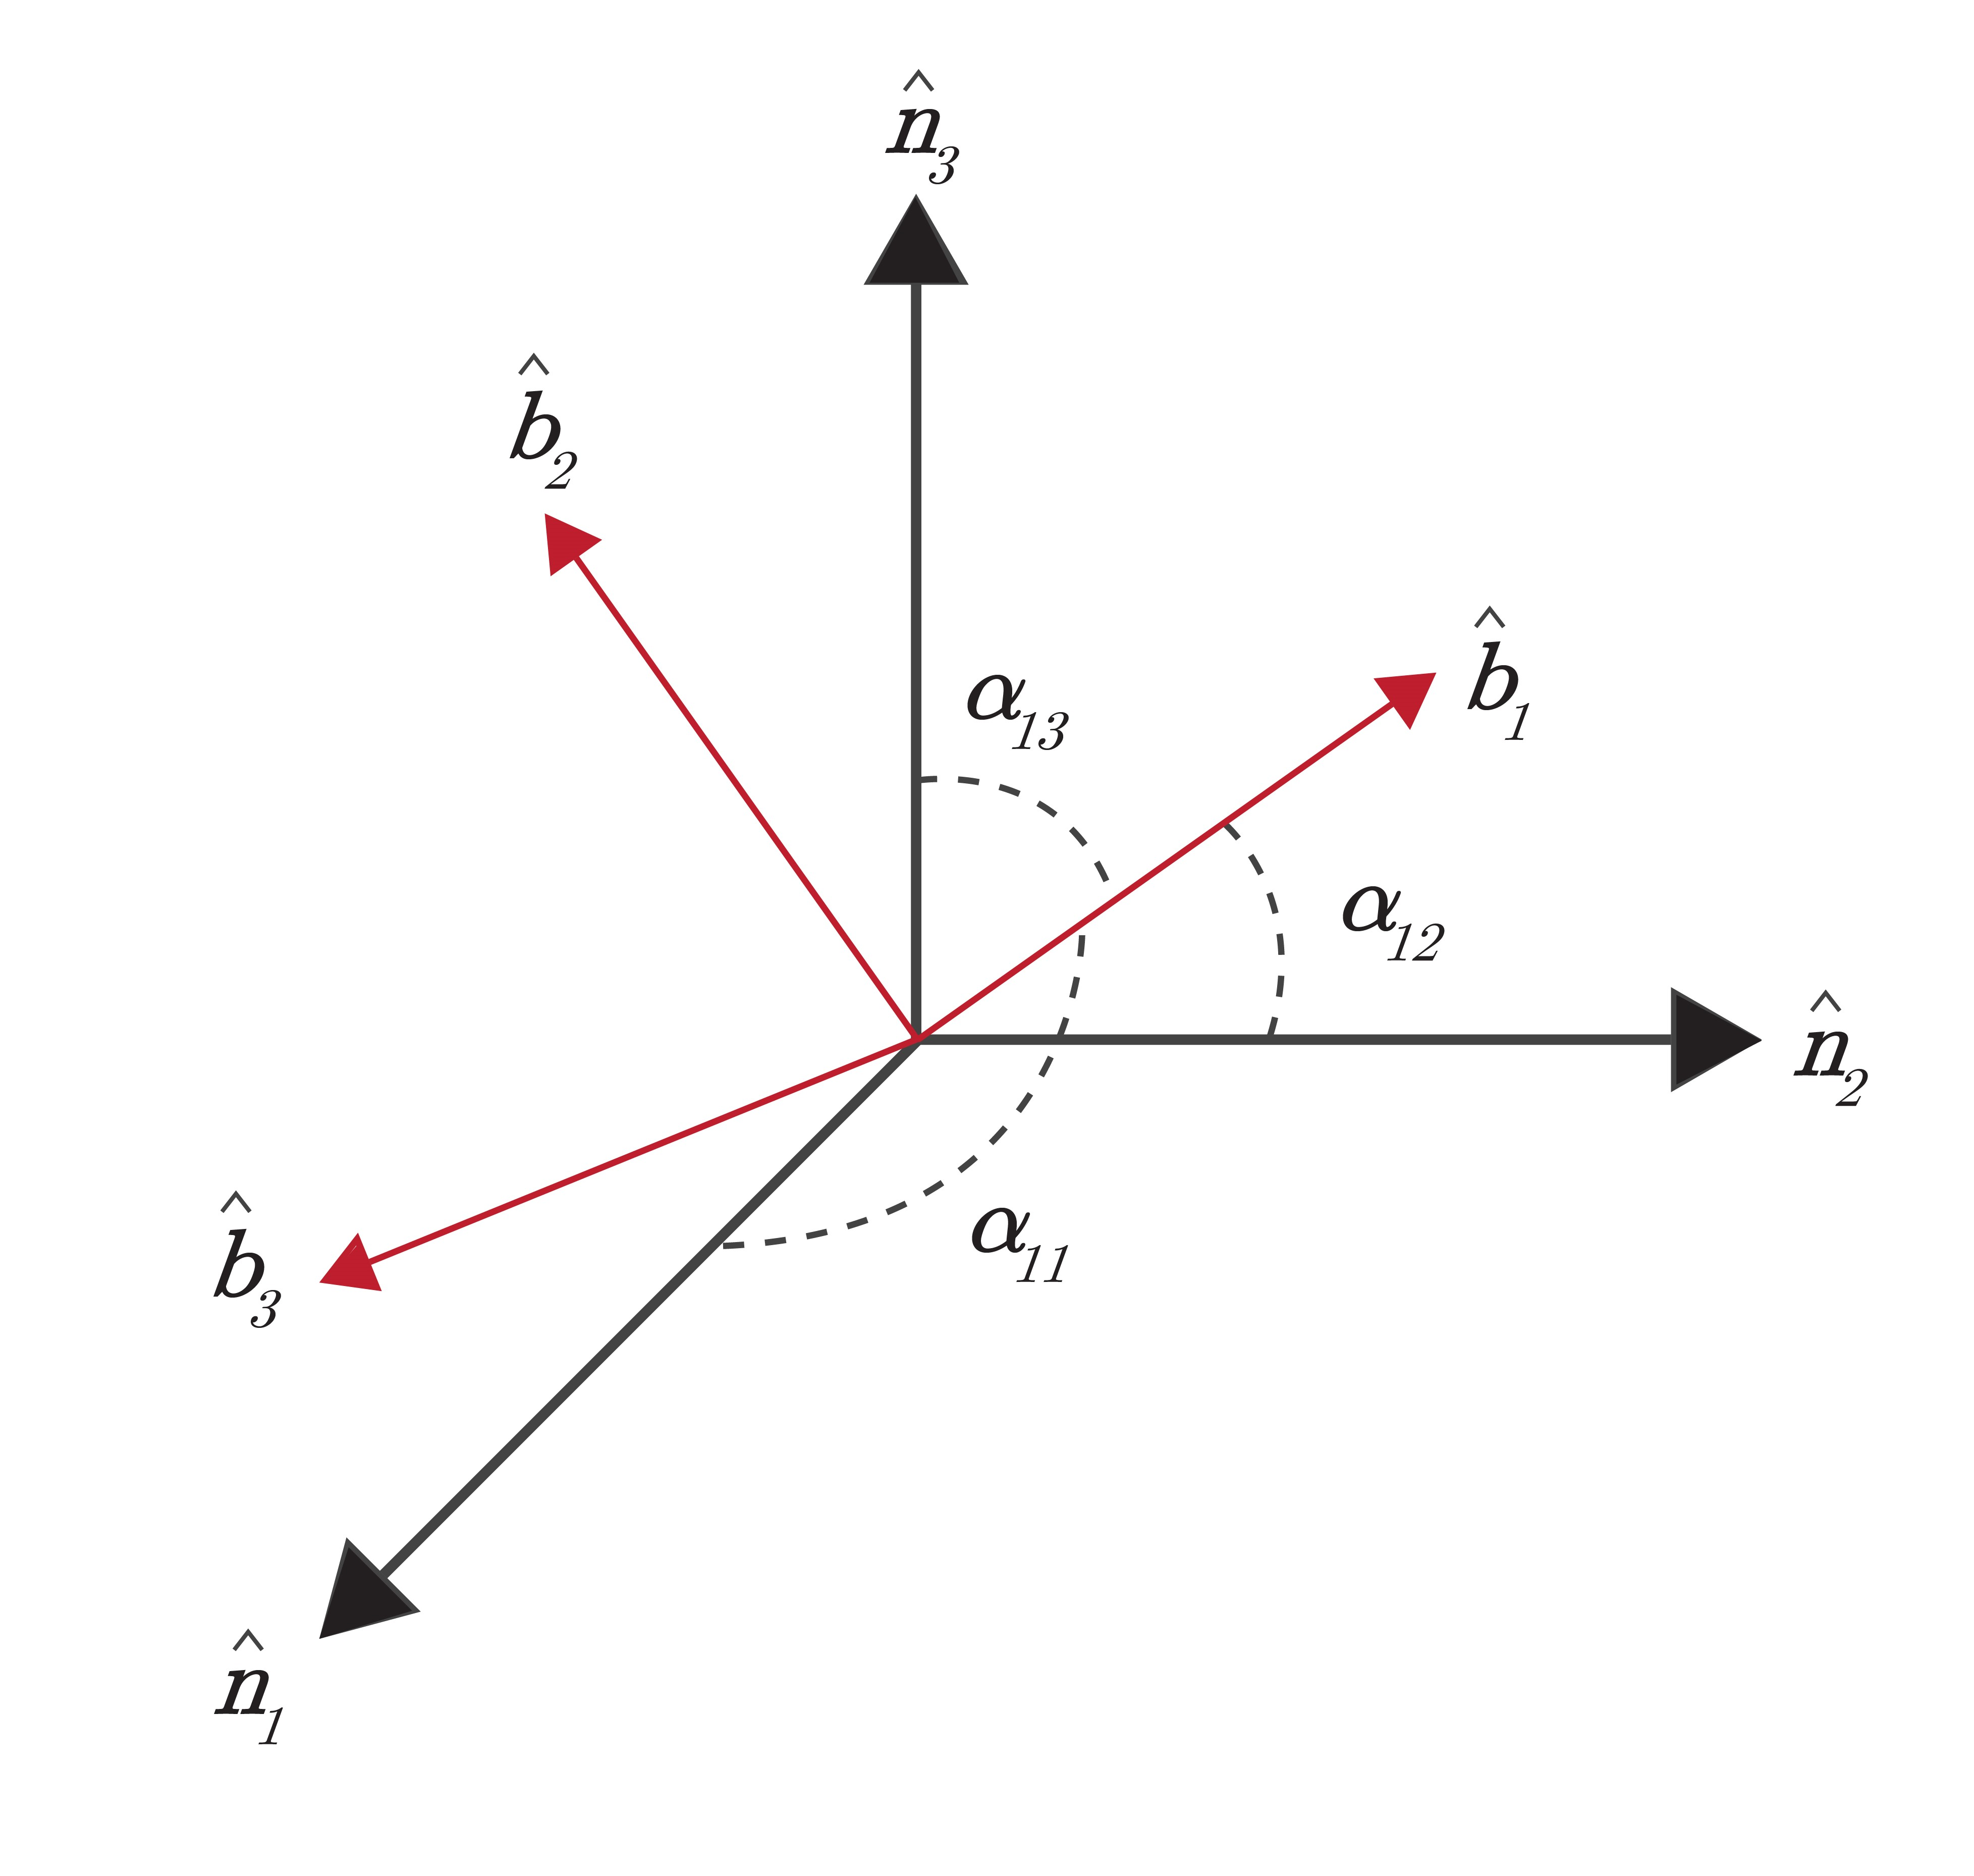
\includegraphics[width=7cm]{dcmalpha}
\end{center}
A good way to relate a body frame vectors to an inertial frame vectors is via the following:

\[\bv{1} = \cos(\alpha_{11})\nv{1} + \cos(\alpha_{12})\nv{2} + \cos(\alpha_{13})\nv{3}\]
\[\bv{2} = \cos(\alpha_{21})\nv{1} + \cos(\alpha_{22})\nv{2} + \cos(\alpha_{23})\nv{3}\]
\[\bv{3} = \cos(\alpha_{31})\nv{1} + \cos(\alpha_{32})\nv{2} + \cos(\alpha_{33})\nv{3}\]
\\
The cosines find the projection of each $\hat{b}$ against each $\hat{n}$. Being masters of linear algebra, we can immediately organize this whole thing into the following, to convert from inertial to body frame:

\[
\{\hat{b}\} = \begin{bmatrix}
\cos(\alpha_{11})&\cos(\alpha_{12})&\cos(\alpha_{13}) \\
\cos(\alpha_{21})&\cos(\alpha_{22})&\cos(\alpha_{23}) \\
\cos(\alpha_{31})&\cos(\alpha_{32})&\cos(\alpha_{33})
\end{bmatrix} \{\hat{n}\} = [BN] \{\hat{n}\}
\]
And from the definition of a cosine, we can also say:
\[
\{\hat{b}\} = \begin{bmatrix}
b_1 \cdot n_1 & b_1 \cdot n_2 & b_1 \cdot n_3 \\
b_2 \cdot n_1 & b_2 \cdot n_2 & b_2 \cdot n_3 \\
b_3 \cdot n_1 & b_3 \cdot n_2 & b_3 \cdot n_3
\end{bmatrix} \{\hat{n}\} = [BN] \{\hat{n}\}
\]
We'll call this matrix [BN]. The BN matrix we have here is the \emph{Direction Cosine Matrix}. It doesn't take a rocket scientiest to see that the ``Direction Cosine" part of the name comes from all these cosines. DCMs are basically glorified rotation matrices.

\subsection{Well, Whats The Point?}
Glad you asked. Here's a situation: You are on Earth and your friend is on a spaceship in orbit. You just saw a really cool star and want to radio up to your friend where to look, with respect to their frame. You know the DCM that converts from your frame to theirs. How would you achieve this?

If it wasn't obvious, it's via that DCM you have. Lets say that v is the vector to the star. We can describe it in both the inertial frame and body frame, like so:
\[v = v_{b1}\bv{1}+v_{b2}\bv{2}+v_{b3}\bv{3}=[v_b]^T\{\hat{b}\}\;(1)\]
\[v = v_{b1}\nv{1}+v_{n2}\nv{2}+v_{n3}\nv{3}=[v_n]^T\{\hat{n}\}\;(2)\]
The $[v_b]$ and $[v_n]$ just indicate the coefficients that you multiply your basis vectors by. That T in the right side of the equation just indicates a transpose. All in all, real standard coordinate frame stuff. 

Well, we have that \{b\} vectrix in the equation 1 and we know that $\{\hat{b}\} = [BN]\{\hat{n}\}$. So lets get to substituting.
\[[v_b]^T\{\hat{b}\} = [v_n]^T\{\hat{n}\}\]
\[[v_b]^T[BN]\{\hat{n}\} = [v_n]^T\{\hat{n}\}\]
Doing some funky transposing and linear algebra things, we'll discover that:
\[\bm{v_b = [BN]v_n}\]
and likewise,
\[\bm{v_n = [BN]^Tv_b}\]
As you can see, DCMs not only \emph{help describe how one frame is rotated relative to another}, but it can also help \emph{translate what one vector looks like to an observer in a different frame}.
\section{Adding and Subtracting DCMs}
Despite all we've been doing so far, we are allowed to have more than 2 frames. For example, let's say your UFO is floating outside the ISS. You know the DCM that converts the ISS frame to your UFO frame. You also know the DCM that converts some inertial frame to ISS frame. What if you want to know how to convert from inertial straight to UFO frame? 

Lets represent the UFO frame as U, the ISS frame as I, and the inertial frame to N. We want to find the DCM [UN], but we only know [UI] and [IN]. The solution is super simple:
\[\bm{[UN] = [UI][IN]}\]

This is what we call \emph{DCM Addition.} But what about \emph{DCM Subtraction}?

Let's say we already know [UN] and we know [IN]. How would we find the UFO frame relative to the ISS frame [UI]? Following our addition we can say:
\[[UI] = [UN][NI]\]
But wait a second, we don't know [NI]? We actually do. Transposing an orthogonal matrix gives the inverse.
\[[IN]^T = [NI]\]
Thus we can say:
\[\bm{[UI] = [UN][IN]^T}\]
Doing this to [UN] subtracts out the part where I is related to N.
\section{Properties}
Well, what makes a DCM a DCM?
\begin{enumerate}
\item{\textbf{DCMs are 3x3}}

\item{\textbf{The magnitude of each row and column is 1.}}

Ensuring the rows and columns are unit length makes the math less chaotic. Let's say that some malevolent DCM doesn't maintain unit length. When you multiply some vector through this DCM, the vector that comes out on the other side isn't the same length as the original. And now, not only do you have to keep track of a ton of numbers, you have to scale that vector's components up or down. Since we want to make our lives as easy as possible, this ain't the move.

\item{\textbf{Every DCM element is $\leq |1|$}}

A consequence of the above. Not exactly hard to see why.

\item{\textbf{DCMs are orthogonal}}

Using vetrices with orthogonal vectors is convention because they're mathematically friendly. The fact that a DCM is orthogonal is the reason we can use the transpose to transform backwards from body to inertial. The inverse of an orthogonal matrix is just its transpose after all.

\item{\textbf{The determinant of a DCM is $\pm 1$ (Unit, Orthogonal)}}

This property is essentially a result of the previous properties piled together. A unit orthogonal matrix has a determinant of $\pm 1$. Why $\pm 1$ you ask? Well the sign of the determinant indicates the handedness of the DCM. A +1 indicates a right handed frame and -1 is a left handed frame. A left handed frame technicallyyyyy isn't wrong, but right handed frames are convention. That's why right handed frames are referred to as ``proper" and left, ``improper".

\item{\textbf{DCMs are non-singular!}}

There's no divisions by zero, no weird functions, and since we're working at the lowest level, not many ambiguities can arise.
\end{enumerate}

\subsection{Wait a Minute...}
If DCMs are non-singular, why don't we exclusively use them to describe attitude? While DCMs are lovely and non-singular, they're not always the easiest/intuitive paramaterization to use. 


The sheer amount of elements in the DCM is not very convenient. 9 elements to keep track of attitude? With properties that we constantly have to enforce? Tacking on angular velocity $\omega$ and multiple frames, the amount of numbers flying around can quickly get out of hand.

DCMs aren't super easy to visualize. If I hand you a list of 9 numbers, would you be able to immediately tell how the body frame is rotated? Probably not.

However, the DCM is super useful for translating between attitude parameterizations.

\section{Test Your Knowledge}
\begin{enumerate}
\item Identify the illegal DCMs:\\\\
	$
	a.
	\begin{bmatrix}
			1&0&0\\
			1&0&0\\
			0&1&0
	\end{bmatrix} 
	b.	
	\begin{bmatrix}
			2&0&0\\
			0&2&0\\
			0&0&2
	\end{bmatrix}
	c.	
	\begin{bmatrix}
			1&0&0\\
			0&0.866&-0.5\\
			0&0.5&0.866
	\end{bmatrix}
	d.
	\begin{bmatrix}
			-1&0&0\\
			0&-1&0\\
			0&0&1
	\end{bmatrix}$ 
\item{Given DCMs [KB], [KJ], [NJ], how would you find DCM [BN]?}
\end{enumerate}

\chapter{Euler Angles}

If you've heard of yaw pitch or roll, you've most certainly heard of Euler Angles.
\begin{center}
\textbf{EULER ANGLES: A parameterization that describes attitude in 3 sequential rotations.}
\end{center}

The definition is pretty self explanatory. To describe an attitude in Euler angles, you need to specify your type of Euler angle, referred to as a \emph{set}. Then, you specify the degrees of the angles that belong to this set. Each of the angles describe how far you rotate the frame around that specified axis. 

Here's a visual example if it ain't too clear:

\begin{center}
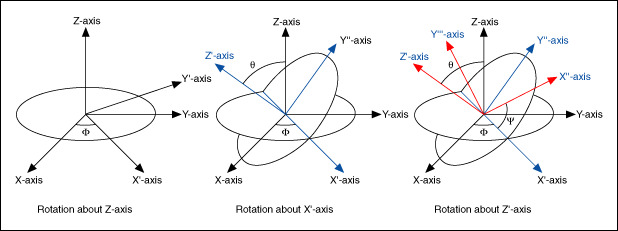
\includegraphics[width=16cm]{euler_proper}
\end{center}

This is what's described as a 3-1-3 Euler Angle, since the rotations operate on the Z, X, and Z body axes. The rotation sequence does the following:
\begin{enumerate}
\item Rotate the frame around the Z-axis by angle $\phi$. This forms a new frame with $X'$ and $Y'$ axes.
\item Rotate the frame around the X'-axis by angle $\theta$. This forms a frame with the $Z'$ and $Y''$ axes.
\item Finally, rotate the frame around the Z' axis by angle $\psi$. This forms a frame with the $X''$ and $Y'''$ axes, and the rotation is finished.
\end{enumerate}

Of course, this is not the only set out there.

\section{Types of Euler Angles}
Euler angles fall into two categories.

\begin{enumerate}
\item{\textbf{Symmetric:}

A Symmetric Euler set implies that the first and last rotation axes are repeated. The best example of this is the 3-1-3 Euler angle shown above.}

\item{\textbf{Asymmetric:}

On the other hand, Asymmetric Euler sets don't have repeating rotation axes. You're probably most familiar with the Yaw-Pitch-Roll or 3-2-1 set.}
\end{enumerate}

In total, there are 12 possible sets.
\section{Euler Angles to DCMs}
Euler Angles relate to DCMs pretty seamlessly. We can represent each individual rotation around an axis as a DCM. These individual rotations just move us from intermediate frame to intermediate frame. Once you have all these DCMs together, you can just multiply them together to find the overall DCM. 

But how do we represent rotations around axes as DCMs?:
\begin{center}
Rotation matrix around axis 1 (X):
\[[R_1(\theta)] = \begin{bmatrix}
			1&0&0\\
			0&\cos{\theta}&\sin{\theta}\\
			0&-\sin{\theta}&\cos{\theta}
	\end{bmatrix}\]	
Rotation matrix around axis 2 (Y):
\[[R_2(\theta)] = \begin{bmatrix}
		\cos{\theta}&0&-\sin{\theta}\\
		0&1&0\\
		\sin{\theta}&0&\cos{\theta}
	\end{bmatrix}\]
Rotation matrix around axis 3 (Z):
\[[R_3(\theta)] = \begin{bmatrix}
		\cos{\theta}&\sin{\theta}&0\\
		-\sin{\theta}&\cos{\theta}&0\\
		0&0&1
	\end{bmatrix}\]

To get the full DCM of a $\alpha\beta\gamma$ Euler set:
\[[BN(\theta_1,\theta_2,\theta_3)] = [R_\gamma(\theta_3)][R_\beta(\theta_2)][R_\alpha(\theta_1)]\]
\end{center}
(Depending who you work with, $\theta_1,\theta_2,\theta_3$ is the same as $\phi,\theta,\psi$, respectively. It'll vary with who you ask, just make sure you clarify.)
\section{DCMs to Euler Angles}
Converting from DCMs to Euler angles is a more involved process, due to the large variety of sets.
\section{Singularities}
As you've probably heard, Euler angles are prone to throwing singularities when rotated in certain ways.
\section{Test Your Knowledge}

\chapter{Principal Rotation Vectors}

Euler Angles are great and easy to visualize, but you really don't wanna use them for body frames that can tumble head over heels. Let's try something new, something called a Principal Rotation Vector. First, let's internalize \emph{Euler's Principal Rotation Theorem}. it states:

\begin{center}
\textbf{THEOREM: A rigid body can be brought from a start to an end orientation by a single rigid rotation ($\phi$ rad/deg) around some principal axis ($\hat{e}$). This principal axis is fixed in both the start and end orientation.}
\end{center}

\begin{center}
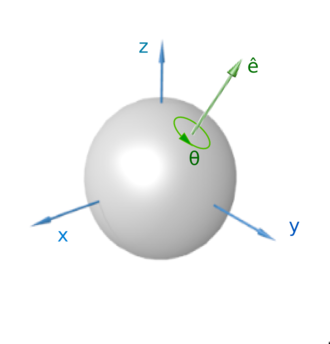
\includegraphics[width=8cm]{PRV1}

(I know it says $\theta$, just pretend it's $\phi$)
\end{center}

We can take advantage of this theorem and derive the \textbf{Principal Rotation Vector} attitude parameterization, also known as \emph{PRVs} for short.\\

PRVs consist of 2 parts:
\begin{enumerate}
\item{\textbf{$\mathbf{\hat{e}}$, The Principal Rotation Vector}

As the name may have revealed, you indeed need to define a principal rotation vector to spin your frame around. The components of the principal rotation vector are labeled as $\mathbf{<e_1, e_2, e_3>}$ }

\item{$\mathbf{\phi}$, \textbf{How Far to Rotate}

You also need to define how far to spin the frame around the PRV.}
\end{enumerate}

\section{PRVs to DCM}
This section isn't too complex, the formula is just thick.
\[[BN] = \begin{bmatrix}
			e_1^2\Sigma+c_\phi&e_1 e_2 \Sigma + e_3 s_\phi&e_1 e_3 \Sigma - e_2 s_\phi\\
			e_2 e_1 \Sigma - e_3 s_\phi&e_2^2 \Sigma + c_\phi&e_2 e_3 \Sigma + e_1 s_\phi\\
			e_3 e_1 \Sigma + e_2 s_\phi&e_3 e_2 \Sigma - e_1 s_\phi&e_3^2 \Sigma + c_\phi
	\end{bmatrix}\]	
\[
\Sigma = 1-c_\phi
\]
Note that the $c_\phi,s_\phi$ are just shorthand for $\cos{\phi},\sin{\phi}$
\section{DCM to PRVs}
Thankfully, this process is a little slimmer.

\[
cos(\phi) = \dfrac{1}{2}(C_{11}+C_{22}+C_{33}-1)
\]
\[
\hat{e} = \begin{bmatrix}
e_1\\e_2\\e_3\\
\end{bmatrix} = \dfrac{1}{2\sin{\phi}}
\begin{bmatrix}
C_{23}-C_{32}\\C_{31}-C_{13}\\C_{12}-C_{21}\\
\end{bmatrix}
\]
\chapter{Quaternions/EPs}

Googling ``quaternion math" will probably scare you, so let's leave all that fancy stuff for the math majors. Taken in the context of PRVs however, they're actually pretty straightforward.

Just to get this out of the way, you'll probably hear the term ``Euler Parameters" being used (EPs for short) and you might wonder what the difference is. Quaternions are the mathematical construct and Euler Parameters are the \emph{coefficients} of the quaternion.\\
 
\section{Well, What is a Quaternion?}
Quaternions form a number system that extends the complex number system. It was invented by William Rowan Hamilton back in 1843, after having an epiphany on a bridge near his home in Ireland. They're usually represented with 4 terms:
\[
a + bi + cj + dk
\]
Where a,b,c,d are real coefficients and i,j,k are hypercomplex. I'm not gonna go deeper into this since I'm certainly not qualified enough to say more.

\section{Defining EPs from PRVs}
As you probably know, quaternions involve 4 terms. We'll refer to them as:
\[<\beta_0,\beta_1,\beta_2,\beta_3>\]
Where $\beta_0$ is the real term. The nomenclature will change according to who you ask, so just make sure you clarify.

Referring back to PRVs, we can define the EPs as:

\[\beta_0 = cos(\phi/2)\]
\[\beta_1 = e_1 sin(\phi/2)\]
\[\beta_2 = e_2 sin(\phi/2)\]
\[\beta_3 = e_3 sin(\phi/2)\]

\section{Constraints}
EPs have only 1 constraint, which is the following:\

\[\beta_0^2+\beta_1^2+\beta_2^2+\beta_3^2=1\]

In math words, this tells us that EPs live on a \emph{unit hypersphere}. Quaternions aren't actually limited to being unit length, but that's a whole nother can of worms that most engineers don't bother opening.
\section{EPs to DCM}
Converting an EP set to a DCM involves the following:
\[
[C] = 
\begin{bmatrix}
\beta_0^2+\beta_1^2-\beta_2^2-\beta_3^2&&2(\beta_1\beta_2+\beta_0\beta_3)&&2(\beta_1\beta_3-\beta_0\beta_2\\
2(\beta_1\beta_2-\beta_0\beta_3)&&\beta_0^2-\beta_1^2+\beta_2^2-\beta_3^2&&2(\beta_2\beta_3+\beta_0\beta_1)\\2(\beta_1\beta_3+\beta_0\beta_2)&&2(\beta_2\beta_3-\beta_0\beta_1)&&\beta_0^2-\beta_1^2-\beta_2^2+\beta_3^2
\end{bmatrix}
\]
If you want a cleaner looking formula,
\[
[BN] = (\beta_0^2 - \epsilon^T\epsilon)[I_{3x3}]+2\epsilon\epsilon^T-2\beta_0[\tilde{\epsilon}]
\]
\[
\epsilon = (\beta_1,\beta_2,\beta_3)
\]
\chapter{Classical Rodriquez Parameters}
Classical Rodriguez Parameters, or CRPs for short, are a 3 coordinate parameterization. These will come in handy when we discuss the QUEST method. In the context of the other parameterizations, they're honestly not all that complex.
\section{EPs to CRPs}
In the context of EPs, CRPs are described as:
\[
q_i = \dfrac{\beta_i}{\beta_0}
\]
for \(i=1,2,3\)
\subsection{A Singularity?}
Your keen eye might have noticed a zero appearing if your angle hits 180. And it's true, \textbf{CRPs hit a singularity when they're pointed at 180 degrees}, like so:
\[
q_i = \dfrac{\beta_i}{\cos(180^{\circ}/2)} = \dfrac{\beta_i}{0}
\]
\section{CRPs to EPs}
\[
\beta_0 = \dfrac{1}{\sqrt{1+q^Tq}}
\]
\[
\beta_i = \dfrac{q_i}{\sqrt{1+q^Tq}}
\]
for \(i=1,2,3\)
\section{PRVs to CRPS}
The relation between CRPs and PRVs is very simple:
\[
\bar{q} = \tan{(\dfrac{\phi}{2})}\hat{e}
\]
For small angles, we can even approximate it to where it's even simpler:
\[
\bar{q} \approx \dfrac{\phi}{2}\hat{e}
\]
\chapter{Attitude Determination?}
Now that you got a good chunk of the preliminaries out of the way, let's get into how it's applied. The whole idea of \emph{Attitude Determination} is broken up into 2 types of problems:
\begin{enumerate}
\item{
\textbf{Static Attitude Determination:} You take all of your measurements at the same time, and try to solve for the optimal geometry of the measurements, figuring out your attitude at that instant of time.
}
\item{\textbf{Dynamic Attitude Determination:} You take your measurements over time and try to figure out how your body is spinning around. This is a far harder problem and one that this text will not cover.
}
\end{enumerate}


\chapter{TRIAD Method}
Published in 1964, TRIAD is one of the oldest algorithms out there. Despite its age, it is still a viable method for simpler satellites.
\chapter{What is Wahba's Problem?}
\section{Definitions and Things}
TRIAD is great and all, but what if we want to make use of all the sensors we have on our satellite? After all, your sponsor would probably be pissed if they paid for a GPS receiver and 4 star trackers but you're only using 1 star tracker and a sun sensor.

\emph{Wahba's problem} was a question posed by the venerable Grace Wahba back in 1965. It goes a little like this:
\subsection{Defining Wahba's Problem}
Assume that we have $n>1$ measurement vectors in body frame ($\vk{B}$) and their corresponding measurement vectors in inertial frame ($\vk{N}$). Attitude determination is basically a problem of finding a $[BN]$ that converts the inertial measurements to the body measurements like so:
\begin{center}
\[
\vk{B}= [\tilde{B}N]\vk{N}
\]
for k = 1,2, ... n
\end{center}
Nothing we don't know (see 3.2.1). However, the real world is mathematically cruel. You will never find a $[\tilde{B}N]$ matrix that perfectly maps from inertial to body, hence the little tilde on the B. This is usually due to imperfect sensors giving imperfect measurement vectors. 

Well, what do we do now? If we can't acquire a perfect [BN], then we should at least try finding a [BN] that maps our inertial measurements as closely as possible to our body measurements. 

So Wahba proposed, ``Hey, why don't we try to minimize this loss function to get the best possible [BN] matrix?"\footnote{I'm pretty sure she didn't actually say this, just roll with it.}:

\[
\mathbf{
J([\tilde{B}N]) = \dfrac{1}{2} \sum^n_{k=1} w_k |\vk{B} - [\tilde{B}N]\vk{N}|^2}
\]

Let's break this down.
\begin{itemize}
\item{$J([\tilde{B}N])$: This describes the overall "wrongness" of the [BN] matrix we're looking at. Smaller J = Better [BN].
}
\item{$w_k$: This is a \emph{weighting value} assigned to that kth measurement vector. You assign this to each sensor yourself. Higher weights are assigned to more reliable sensors. For example, you would assign a higher weight to a sun sensor or star tracker vs a magnetometer. Note that only relative sizes of the weight values matter, the actual values themselves don't really matter.
}
\item{$\hat{v}_k^B - [\tilde{B}N]\hat{v}_k^N$: This describes the error between the kth body measurement and the corresponding kth inertial measurement, mapped to body.}
\end{itemize}

When you boil it down, it's basically a fancier least squares fit. Finding a solution involves minimizing the J as much as possible.

\subsection{Well, How Do We Solve It?}
Actually, there's no one definitive way to solve this. In addition, clever mathematicians and engineers are still coming up with solutions.
\chapter{Davenport's Q}
The first solution to Wahba's problem we're gonna look at is called Davenport's Q. Paul B. Davenport came up with this quaternion based method in 1968. It is an older method, but it is a precursor to other methods out there, like QUEST. 

Beware, this chapter will get a bit math heavy. If you don't feel like looking at the derivation, just check out the ``In a Nutshell" section and cherry pick the formulas.

\subsection{Wahba's Problem in Another Light}
Instead of outright trying to minimize J, we can twist Wahba's problem into another form, in which we can minimize a value called the "gain". Let's see how it's done. 

This is the normal definition of Wahba's problem.
\[
J([\tilde{B}N]) = \dfrac{1}{2} \sum^n_{k=1} w_k |\vk{B} - [\tilde{B}N]\vk{N}|^2
\]
That squared part in the right hand side is the same as taking a dot product, so let's just replace it:
\[
J([\tilde{B}N]) = \dfrac{1}{2} \sum^n_{k=1} w_k (\vk{B} - [\tilde{B}N]\vk{N})^T(\vk{B} - [\tilde{B}N]\vk{N})
\]
Evaluating this dot product mish mash gives us:
\[
J([\tilde{B}N]) = \dfrac{1}{2} \sum^n_{k=1} w_k (\vk{B}^T\vk{B}+\vk{N}^T\vk{N}-2\vk{B}^T[\tilde{B}N]\vk{N})
\]
Continuing to evaluate and simplify gives us:
\[
J([\tilde{B}N]) = \sum^n_{k=1} w_k (1- \vk{B}^T[\tilde{B}N]\vk{N})
\]
Don't worry, this is just Wahba's cost function, just in a different form. We still want to minimize J so how do we go about this? We'll have to maximize $$\vk{B}^T[\tilde{B}N]\vk{N}$$ We remake this as the \textbf{``gain"}:
\[
\mathbf{
g = \sum^n_{k=1} w_k (\vk{B}^T[\tilde{B}N]\vk{N})}
\]
\emph{In order to minimize J, we have to maximize the gain, g.}

\section{Davenport's Method}
Davenport developed the following way to get a gain function in the context of quaternions. Bear with me, this is quite the batch of equations.

\[
[B] = \sum^N_{k=1} w_k\vk{B}\vk{N}^T
\]
\[
[Z] = [(B_{23}-B_{32}), (B_{31}-B_{13}), (B_{12}-B_{21})]^T
\]
\[
\sigma = trace([B])
\]
\[
[S] = [B]+[B]^T
\]
\[
[K] =
\begin{bmatrix}
\sigma && Z^T \\ Z && S-\sigma  [I_{3x3}]
\end{bmatrix}
\]
Finally,
\[
g(\tilde{\beta}) = \bar{\beta}^T[K]\bar{\beta}
\]
Where
\[\bar{\beta} = <\beta_0,\beta_1,\beta_2,\beta_3>\]
\subsection{Maximizing the Gain?}
We are still trying to maximize gain, so we could simply go ``Let's just boost $\bar{\beta}$ to infinity". While a good first thought, this won't work since we have to honor the \emph{constraint} that EPs must be unit length. This has turned into a constrained optimization problem. A good way to solve constrained optimization problems is via Lagrange Multipliers, as you may (or may not) remember from Calc 3. Let's represent our Lagrangified gain formula as $g'$.
\[
g'(\bar{\beta}) = \underbracket{\bar{\beta}^T[K]\bar{\beta}}_{g} - \underbracket{\lambda(\bar{\beta}^T\bar{\beta}-1)}_{constraint}
\]
We'll need to differentiate $g'$ in order to find the extremum:
\[
\dfrac{d(g'(\bar{\beta}))}{d\bar{\beta}} = 2[K]\bar{\beta} - 2\lambda\bar{\beta}=0
\]
As you can clearly see, what comes out is an eigenvector problem:
\[
[K]\bar{\beta}=\lambda\bar{\beta}
\]
Well, what does this mean for us? The gain formula just turns into:
\[
g(\bar{\beta}) = \bar{\beta}^T[K]\bar{\beta} = \bar{\beta}^T\lambda\bar{\beta} = \lambda
\]Therefore, the optimal EP set is the eigenvector associated with the largest eigenvalue of K.
\section{In a Nutshell}

To summarize, Davenport's Q boils down to the following:
\begin{enumerate}
\item{Compute the [K] matrix.}
\item{Find the eigenvalues and eigenvectors of said [K] matrix.}
\item{Choose the largest eigenvalue + corresponding eigenvector.}
\item{This eigenvector is your set of EPs.}
\end{enumerate}


\chapter{QUEST}
Davenport's Q is lovely, but computationally, solving that eigenvalue problem is computationally expensive. This makes it fairly unpopular for realtime applications. In order to gain a bit of speed, how about we cleverly tackle that eigenvalue problem a different way? Although a little less straightforward, the extra speed offered by QUEST (which stands for QUaternion ESTimation) is much appreciated. Like the Davenport's Q chapter, quite math heavy.
\section{A Nice Approximation}
Recall from the previous chapter the loss ($J$) and gain ($g$) functions:
\[
J([\tilde{B}N]) = \sum^n_{k=1} w_k (1- \vk{B}^T[\tilde{B}N]\vk{N})
\]
\[
g = \sum^n_{k=1} w_k (\vk{B}^T[\tilde{B}N]\vk{N})
\]
Also recall that the gain function eventually comes out to be the K matrix's largest eigenvalue, let's call this $\lambda_{opt}$:
\[
g(\bar{\beta}) = \lambda_{opt}
\]
This must mean that, to find an optimal J,
\[
J = \sum^n_{k=1} w_k - g = \sum^n_{k=1} w_k - \lambda_{opt}
\]
Let's isolate the optimal eigenvalue:
\[
\lambda_{opt} = \sum^n_{k=1} w_k - J
\]
Solving the problem like this seems like a whole bunch of work that we don't want to do, so let's just assume J is small. Like really, really small. In fact, so small that we can treat it like 0. Thus, the equation turns into:
\[
\mathbf{
\lambda_{opt} \approx \sum^n_{k=1} w_k
}\]
We now have a \emph{really} good guess at the real optimal eigenvalue. (Well, unless your sensors are throwing laughably bad measurements that is)

\section{Refining the Guess}
We got a great guess, but it's still just a guess. In order to continue, we need to refine it and numerically find the actual maximum eigenvalue. We know that eigenvalues must satisfy the characteristic equation:
\[
f(s) = det([K]-s[I_{3x3}]) = 0
\]
If this seems a tad unfamiliar, just think back on how you found the eigenvalues for a 2 x 2 matrix. An example:
\[
det(
\begin{bmatrix}
0&&1\\-2&&-3
\end{bmatrix} - 
\begin{bmatrix}
\lambda&&0\\0&&\lambda
\end{bmatrix}) = 0
\]
Which gives a characteristic equation of
\[
\lambda^2+3\lambda+2=0
\]
Since we're trying to find the root of the characteristic equation, we can use Newton-Raphson iteration. Newton-Raphson is just a numerical method to find the roots of polynomials. Don't let the "numerical" scare you, it's actually pretty simple. We'll use the $f(s)$  (the characteristic equation) we defined above and its derivative in the Newton-Raphson:
\[
\lambda_0 = \sum^n_{k=1} w_k
\]
\[
\lambda_1 = \lambda_0 - \dfrac{f(\lambda_0)}{f'(\lambda_0)}
\]
Repeating this process a couple of times and checking whether $\lambda$ fulfills the characteristic equation,
\[
\lambda_{max} = \lambda_i = \lambda_{i-1} - \dfrac{f(\lambda_{i-1})}{f'(\lambda_{i-1})}
\]
Repeating this moves you closer and closer to the actual maximum eigenvalue. We're allowed to do this since our $\lambda_{opt}$ guess already places us close to the actual $\lambda_{max}$.

\section{Searching for \(\bar{q}\)}
QUEST is actually a bit of a misnomer, since we'll actually be first receiving the result in CRPs. A quick refresher on CRPs:
\[
q = \hat{e} \tan{\dfrac{\phi}{2}} = 
\dfrac{1}{\beta_0 }
\begin{bmatrix}
\beta_1\\
\beta_2\\
\beta_3
\end{bmatrix}
\]
And let's describe a convenient notational link between the EPs and CRPs, like so:
\[
\dfrac{\bar{\beta}}{\beta_0} = 
\begin{bmatrix}
1\\\bar{q} 
\end{bmatrix}
\]
First, our original eigenvector problem looks like:
\[
[K]\bar{\beta} = \lambda_{opt}\bar{\beta}
\]
Let's get this whole formula into CRPs and expand the K matrix:
\[
[K]\dfrac{\bar{\beta}}{\beta_0} = \lambda_{opt}\dfrac{\bar{\beta}}{\beta_0}
\]
\[
\begin{bmatrix}
\sigma&&Z^T\\
Z&&S-\sigma[I_{3x3}]
\end{bmatrix}
\begin{bmatrix}
1\\\bar{q} 
\end{bmatrix} = \lambda_{opt}
\begin{bmatrix}
1\\\bar{q} 
\end{bmatrix}
\]
If we do the whole matrix multiplication and just trim out the unnecessary top row, we'll get:
\[
[Z] + ([S] - \sigma [I_{3x3}])\bar{q} = \lambda_{opt}\bar{q}
\]
Superb, we're getting close now. We can now isolate $\bar{q}$, thus:
\[
\mathbf{
\bar{q} = ((\lambda_{opt}+\sigma)[I_{3x3}] - [S])^{-1}[Z]
}
\]
Well, you came for EPs after all, so you'll need to do the following to convert back to EPs.
\[
\bar{\beta} = \dfrac{1}{\sqrt{1+\bar{q}^T\bar{q}}} 
\begin{bmatrix}
1\\\bar{q} 
\end{bmatrix}
\]
\section{Aren't You Forgetting Something?}
If alarm bells are going off in your head since CRPs go singular at 180 degrees, then you are absolutely right. The way this is resolved is by considering an \emph{alternate body frame}, determining your attitude from that, and adjusting afterwards to your true body frame. Having these 2 body frames will ensure that both will not bump into that singularity at the same time. 

This technique is valid since defining a body frame is completely arbitrary. After all, what's stopping you from defining your $b_1$ vector towards say, the left wing of your spaceship?\footnote{The answer is nothing, if you're actually wondering.}
\section{In a Nutshell}
\begin{enumerate}
\item{Estimate \(\lambda_{opt}\) by summing the weight values.}
\item{Refine your \(\lambda_{opt}\) guess by doing Newton-Raphson with the characteristic equation.}
\item{Acquire your optimal attitude in CRPs. Convert to quaternions.}
\item{If need arise, handle the singularity} 
\end{enumerate}
\chapter{Answer Key}
\section{Chapter 1 DCM}
\begin{enumerate}
\item{a \& b}
\item{$[KB]^T[KJ][NJ]^T$}


\end{enumerate}
\end{document}
